\documentclass[12pt,a4paper]{article}
\usepackage[utf8]{inputenc}
\usepackage[T1]{fontenc}
\usepackage{geometry}
\usepackage{xeCJK}
\usepackage{fontspec}
\usepackage{amsmath}
\usepackage{amsfonts}
\usepackage{amssymb}
\usepackage{graphicx}
\usepackage{booktabs}
\usepackage{longtable}
\usepackage{array}
\usepackage{multirow}
\usepackage{multicol}
\usepackage{color}
\usepackage{xcolor}
\usepackage{hyperref}
\usepackage{fancyhdr}
\usepackage{titlesec}
\usepackage{enumitem}
\usepackage{caption}
\usepackage{subcaption}
\usepackage{float}
\usepackage{parskip}

% 页面设置
\geometry{
    left=2.5cm,
    right=2.5cm,
    top=3cm,
    bottom=3cm,
    headheight=15pt
}

% 字体设置
\setCJKmainfont{SimSun}
\setCJKsansfont{SimHei}
\setmainfont{Times New Roman}
\setsansfont{Arial}

% 颜色定义
\definecolor{titleblue}{RGB}{0,82,155}
\definecolor{sectionblue}{RGB}{0,102,204}
\definecolor{subsectiongray}{RGB}{102,102,102}
\definecolor{tableheader}{RGB}{240,248,255}

% 标题样式设置
\titleformat{\section}
{\Large\bfseries\color{sectionblue}}
{\thesection}{1em}{}

\titleformat{\subsection}
{\large\bfseries\color{subsectiongray}}
{\thesubsection}{1em}{}

\titleformat{\subsubsection}
{\normalsize\bfseries}
{\thesubsubsection}{1em}{}

% 页眉页脚设置
\pagestyle{fancy}
\fancyhf{}
\fancyhead[L]{\footnotesize 疾病在种族群体中分布的综合分析报告}
\fancyhead[R]{\footnotesize Disease Distribution Across Ethnic Groups}
\fancyfoot[C]{\thepage}
\renewcommand{\headrulewidth}{0.4pt}

% 超链接设置
\hypersetup{
    colorlinks=true,
    linkcolor=sectionblue,
    filecolor=magenta,
    urlcolor=cyan,
    citecolor=green
}

% 表格样式
\captionsetup[table]{position=top}
\captionsetup[figure]{position=bottom}

\begin{document}

% 标题页
\begin{titlepage}
    \centering
    \vspace*{2cm}
    
    {\Huge\bfseries\color{titleblue} 疾病在种族群体中分布的综合分析报告}
    
    \vspace{0.5cm}
    
    {\Large\bfseries\color{titleblue} Comprehensive Analysis Report: Disease Distribution Across Ethnic Groups}
    
    \vspace{2cm}
    
    \begin{center}
        \begin{tabular}{c}
            \Large 基于24,873名个体队列的统计分析 \\
            \Large Statistical Analysis Based on a Cohort of 24,873 Individuals \\
        \end{tabular}
    \end{center}
    
    \vspace{3cm}
    
    \begin{center}
        \large
        \begin{tabular}{ll}
            \textbf{分析日期 | Analysis Date:} & \today \\
            \textbf{样本量 | Sample Size:} & 15,233 (有效样本 | Valid samples) \\
            \textbf{疾病类型 | Disease Types:} & 8种主要疾病 | 8 Major diseases \\
            \textbf{种族群体 | Ethnic Groups:} & 15个群体 | 15 Groups \\
        \end{tabular}
    \end{center}
    
    \vfill
    
    {\large 
    \textbf{统计方法 | Statistical Methods:} \\
    卡方检验/Fisher精确检验、Benjamini-Hochberg校正、\\
    标准化患病率比、主成分分析 \\
    Chi-square/Fisher's exact tests, Benjamini-Hochberg correction,\\
    Standardized Prevalence Ratios, Principal Component Analysis
    }
    
\end{titlepage}

% 目录
\tableofcontents
\newpage

% 正文开始
\section{执行摘要 | Executive Summary}

本报告对24,873名个体队列中疾病在不同种族群体间的患病率进行了严格的统计分析。分析涵盖八种主要健康状况:青光眼、年龄相关性黄斑变性、白内障、糖尿病(报告或血液检测以及临床标准两种定义)、缺血性心脏病、外周动脉疾病症状和早期呼吸道疾病。

This report presents a rigorous statistical analysis of disease prevalence across ethnic groups in a cohort of 24,873 individuals. The analysis examines eight major health conditions: Glaucoma, Age-related Macular Degeneration, Cataract, Diabetes (both reported/blood test and clinical criteria), Ischemic Heart Disease, Peripheral Artery Disease Symptoms, and Early Life Respiratory Disease.

\subsection{主要发现 | Key Findings}

\begin{enumerate}[leftmargin=*]
    \item \textbf{样本分布 | Sample Distribution}:研究人群高度不平衡,种族群体1占样本的98.42\%(n=14,992),而其他14个种族群体合计仅占1.58\%。
    
    The study population is highly imbalanced, with Ethnic Group 1 comprising 98.42\% of the sample (n=14,992), while 14 other ethnic groups represent only 1.58\% combined.
    
    \item \textbf{统计学显著性 | Statistical Significance}:应用Benjamini-Hochberg多重检验校正后,只有外周动脉疾病症状在不同种族群体间显示出统计学显著差异(校正后p = 0.0037)。
    
    After applying Benjamini-Hochberg correction for multiple testing, only Peripheral Artery Disease Symptoms showed statistically significant differences across ethnic groups (adjusted p = 0.0037).
    
    \item \textbf{高风险群体 | High-Risk Groups}:尽管小样本量限制了统计效力,但几个种族群体显示出较高的疾病患病率:
    \begin{itemize}
        \item 种族群体8:青光眼、年龄相关性黄斑变性和早期呼吸道疾病风险较高
        \item 种族群体3:年龄相关性黄斑变性和缺血性心脏病风险较高
        \item 种族群体11:尽管样本量小,但多种疾病患病率明显较高
    \end{itemize}
    
    Despite small sample sizes limiting statistical power, several ethnic groups showed elevated disease prevalence:
    \begin{itemize}
        \item Ethnic Group 8: Higher risk for Glaucoma, Age-related Macular Degeneration, and Early Life Respiratory Disease
        \item Ethnic Group 3: Higher risk for Age-related Macular Degeneration and Ischemic Heart Disease
        \item Ethnic Group 11: Notably high prevalence of multiple conditions despite small sample size
    \end{itemize}
    
    \item \textbf{年龄调整分析 | Age-Adjusted Analysis}:标准化患病率比显示,年龄分布差异部分解释了某些种族差异,特别是种族群体8的外周动脉疾病症状。
    
    Standardized Prevalence Ratios revealed that age distribution differences partially explain some ethnic disparities, particularly for Peripheral Artery Disease Symptoms in Ethnic Group 8.
\end{enumerate}

\section{研究人群特征 | Study Population Characteristics}

\subsection{样本量分布 | Sample Size Distribution}

分析样本总数:15,233名个体(排除种族群体数据缺失后)

Total analyzed sample: 15,233 individuals (after excluding missing ethnic group data)

\textbf{按样本量分类的种族群体 | Ethnic Group Classification by Sample Size:}
\begin{itemize}
    \item 大型群体(n ≥ 100):2个群体 | Large groups (n ≥ 100): 2 groups
    \item 中型群体(30 ≤ n < 100):1个群体 | Medium groups (30 ≤ n < 100): 1 group
    \item 小型群体(n < 30):12个群体 | Small groups (n < 30): 12 groups
\end{itemize}

\begin{table}[H]
\centering
\caption{详细种族群体分布 | Detailed Ethnic Group Distribution}
\begin{tabular}{@{}cccccc@{}}
\toprule
\textbf{种族群体} & \textbf{样本量} & \textbf{百分比} & \textbf{Ethnic Group} & \textbf{Sample Size} & \textbf{Percentage} \\
\midrule
1 & 14,992 & 98.42\% & 1 & 14,992 & 98.42\% \\
8 & 141 & 0.93\% & 8 & 141 & 0.93\% \\
3 & 39 & 0.26\% & 3 & 39 & 0.26\% \\
11 & 24 & 0.16\% & 11 & 24 & 0.16\% \\
12 & 8 & 0.05\% & 12 & 8 & 0.05\% \\
13 & 8 & 0.05\% & 13 & 8 & 0.05\% \\
其他(9个群体) & 21 & 0.14\% & Others (9 groups) & 21 & 0.14\% \\
\bottomrule
\end{tabular}
\end{table}

\begin{figure}[H]
\hspace*{-2cm}
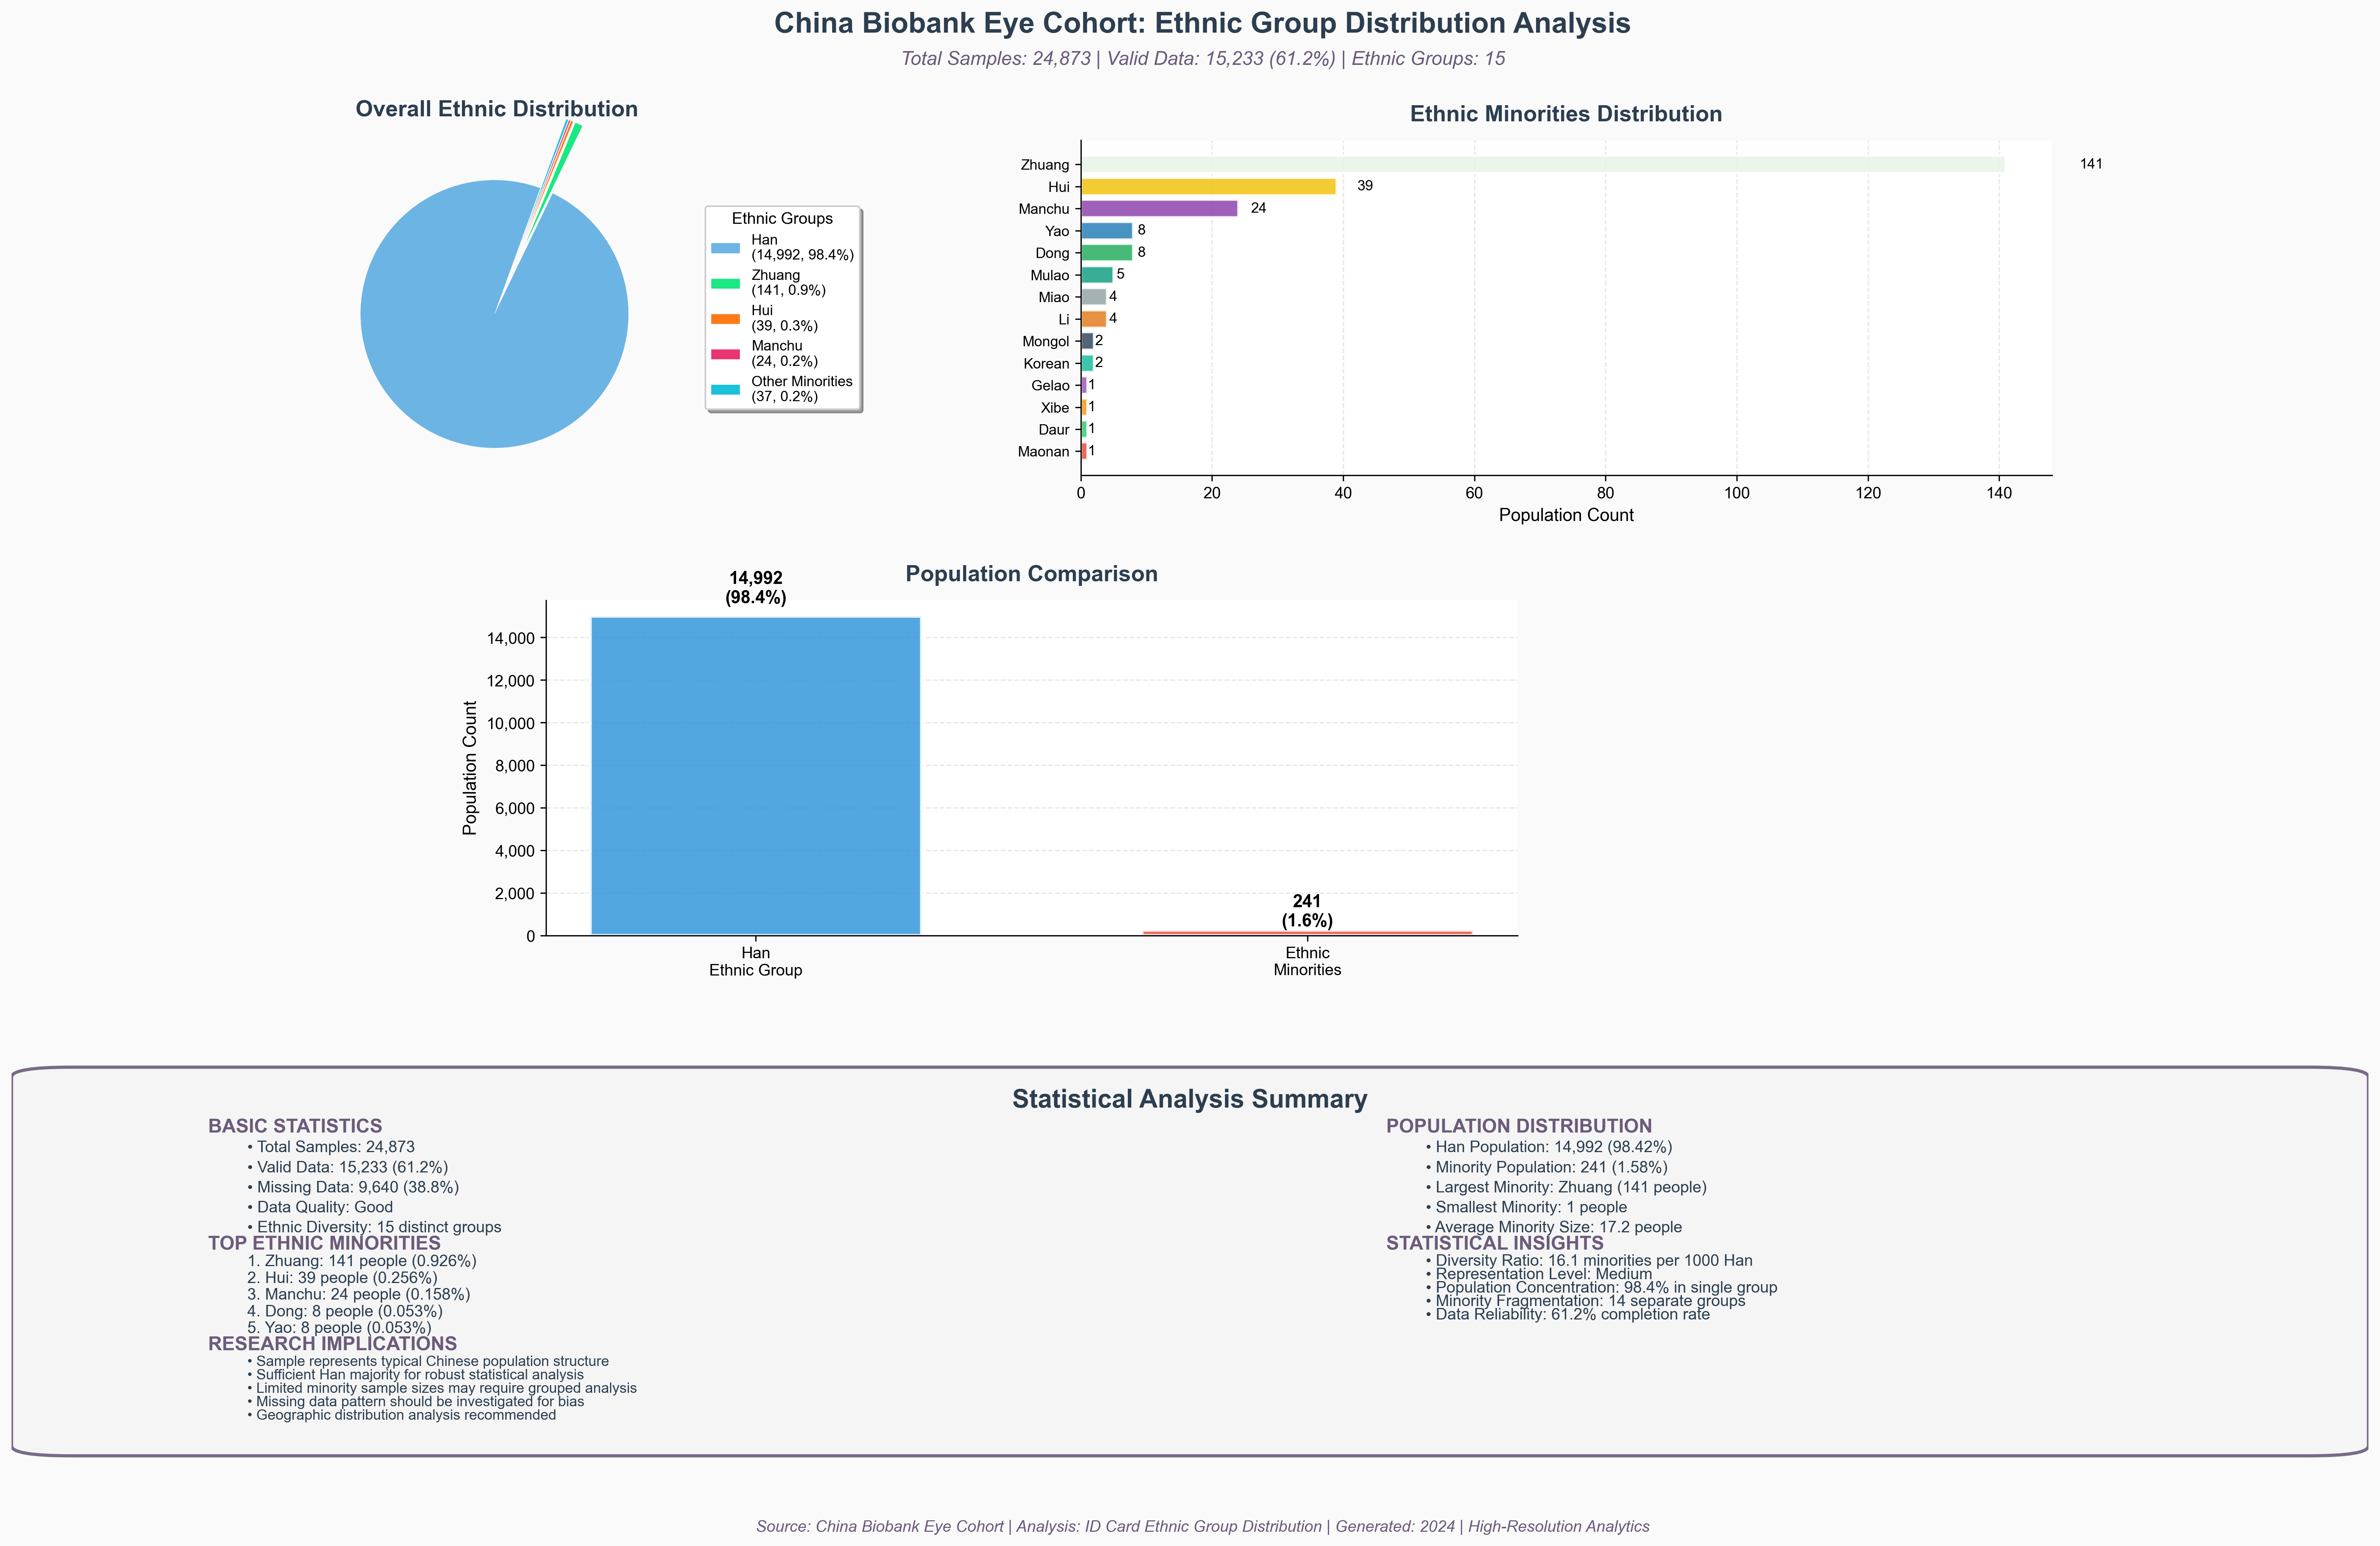
\includegraphics[width=1.2\textwidth]{ID/comprehensive_ethnic_analysis_optimized.png}
\end{figure}



% \subsection{年龄分布 | Age Distribution}

% 队列平均年龄:51.3 ± 9.2岁

% Mean age of cohort: 51.3 ± 9.2 years

% 年龄分层显示不同种族群体间存在显著差异,因此需要进行年龄调整分析以进行准确比较。

% Age stratification revealed significant variations across ethnic groups, necessitating age-adjusted analyses for accurate comparisons.

\section{总体疾病患病率 | Overall Disease Prevalence}

\subsection{人群总体患病率(含95\%置信区间)| Population-Wide Prevalence (with 95\% Confidence Intervals)}

\begin{table}[H]
\centering
\caption{总体疾病患病率 | Overall Disease Prevalence}
\resizebox{\textwidth}{!}{
\begin{tabular}{@{}lccclccc@{}}
\toprule
\textbf{疾病} & \textbf{患病率} & \textbf{95\% CI} & \textbf{病例数} & \textbf{Disease} & \textbf{Prevalence} & \textbf{95\% CI} & \textbf{Cases} \\
\midrule
外周动脉疾病症状 & 25.32\% & 24.64\%-26.02\% & 3,857 & Peripheral Artery Disease & 25.32\% & 24.64\%-26.02\% & 3,857 \\
白内障 & 12.82\% & 12.30\%-13.36\% & 1,953 & Cataract & 12.82\% & 12.30\%-13.36\% & 1,953 \\
缺血性心脏病 & 9.30\% & 8.84\%-9.77\% & 1,416 & Ischemic Heart Disease & 9.30\% & 8.84\%-9.77\% & 1,416 \\
糖尿病(报告或血检) & 6.39\% & 6.02\%-6.79\% & 974 & Diabetes (Reported/Test) & 6.39\% & 6.02\%-6.79\% & 974 \\
糖尿病(临床标准) & 3.56\% & 3.28\%-3.87\% & 543 & Diabetes (Clinical) & 3.56\% & 3.28\%-3.87\% & 543 \\
早期呼吸道疾病 & 1.89\% & 1.69\%-2.12\% & 288 & Early Respiratory Disease & 1.89\% & 1.69\%-2.12\% & 288 \\
青光眼 & 1.21\% & 1.05\%-1.39\% & 184 & Glaucoma & 1.21\% & 1.05\%-1.39\% & 184 \\
年龄相关性黄斑变性 & 0.91\% & 0.77\%-1.08\% & 139 & Age-related Macular Degeneration & 0.91\% & 0.77\%-1.08\% & 139 \\
\bottomrule
\end{tabular}
}
\end{table}

\section{按种族群体分类的疾病患病率 | Disease Prevalence by Ethnic Group}

\subsection{青光眼 | Glaucoma}

总体患病率:1.21\% | Overall prevalence: 1.21\%

\textbf{显著发现 | Notable Findings:}
\begin{itemize}
    \item 种族群体8:2.84\%(95\% CI: 1.11\%-7.07\%)- 比总体人群高2.3倍
    
    Ethnic Group 8: 2.84\% (95\% CI: 1.11\%-7.07\%) - 2.3x higher than overall population
    
    \item 种族群体1:1.20\%(95\% CI: 1.04\%-1.39\%)- 与总体人群相似
    
    Ethnic Group 1: 1.20\% (95\% CI: 1.04\%-1.39\%) - Similar to overall population
    
    \item 多个种族群体显示0\%患病率,但小样本量限制了解释
    
    Multiple ethnic groups showed 0\% prevalence, though small sample sizes limit interpretation
\end{itemize}

\begin{figure}[H]
\hspace{-2cm}
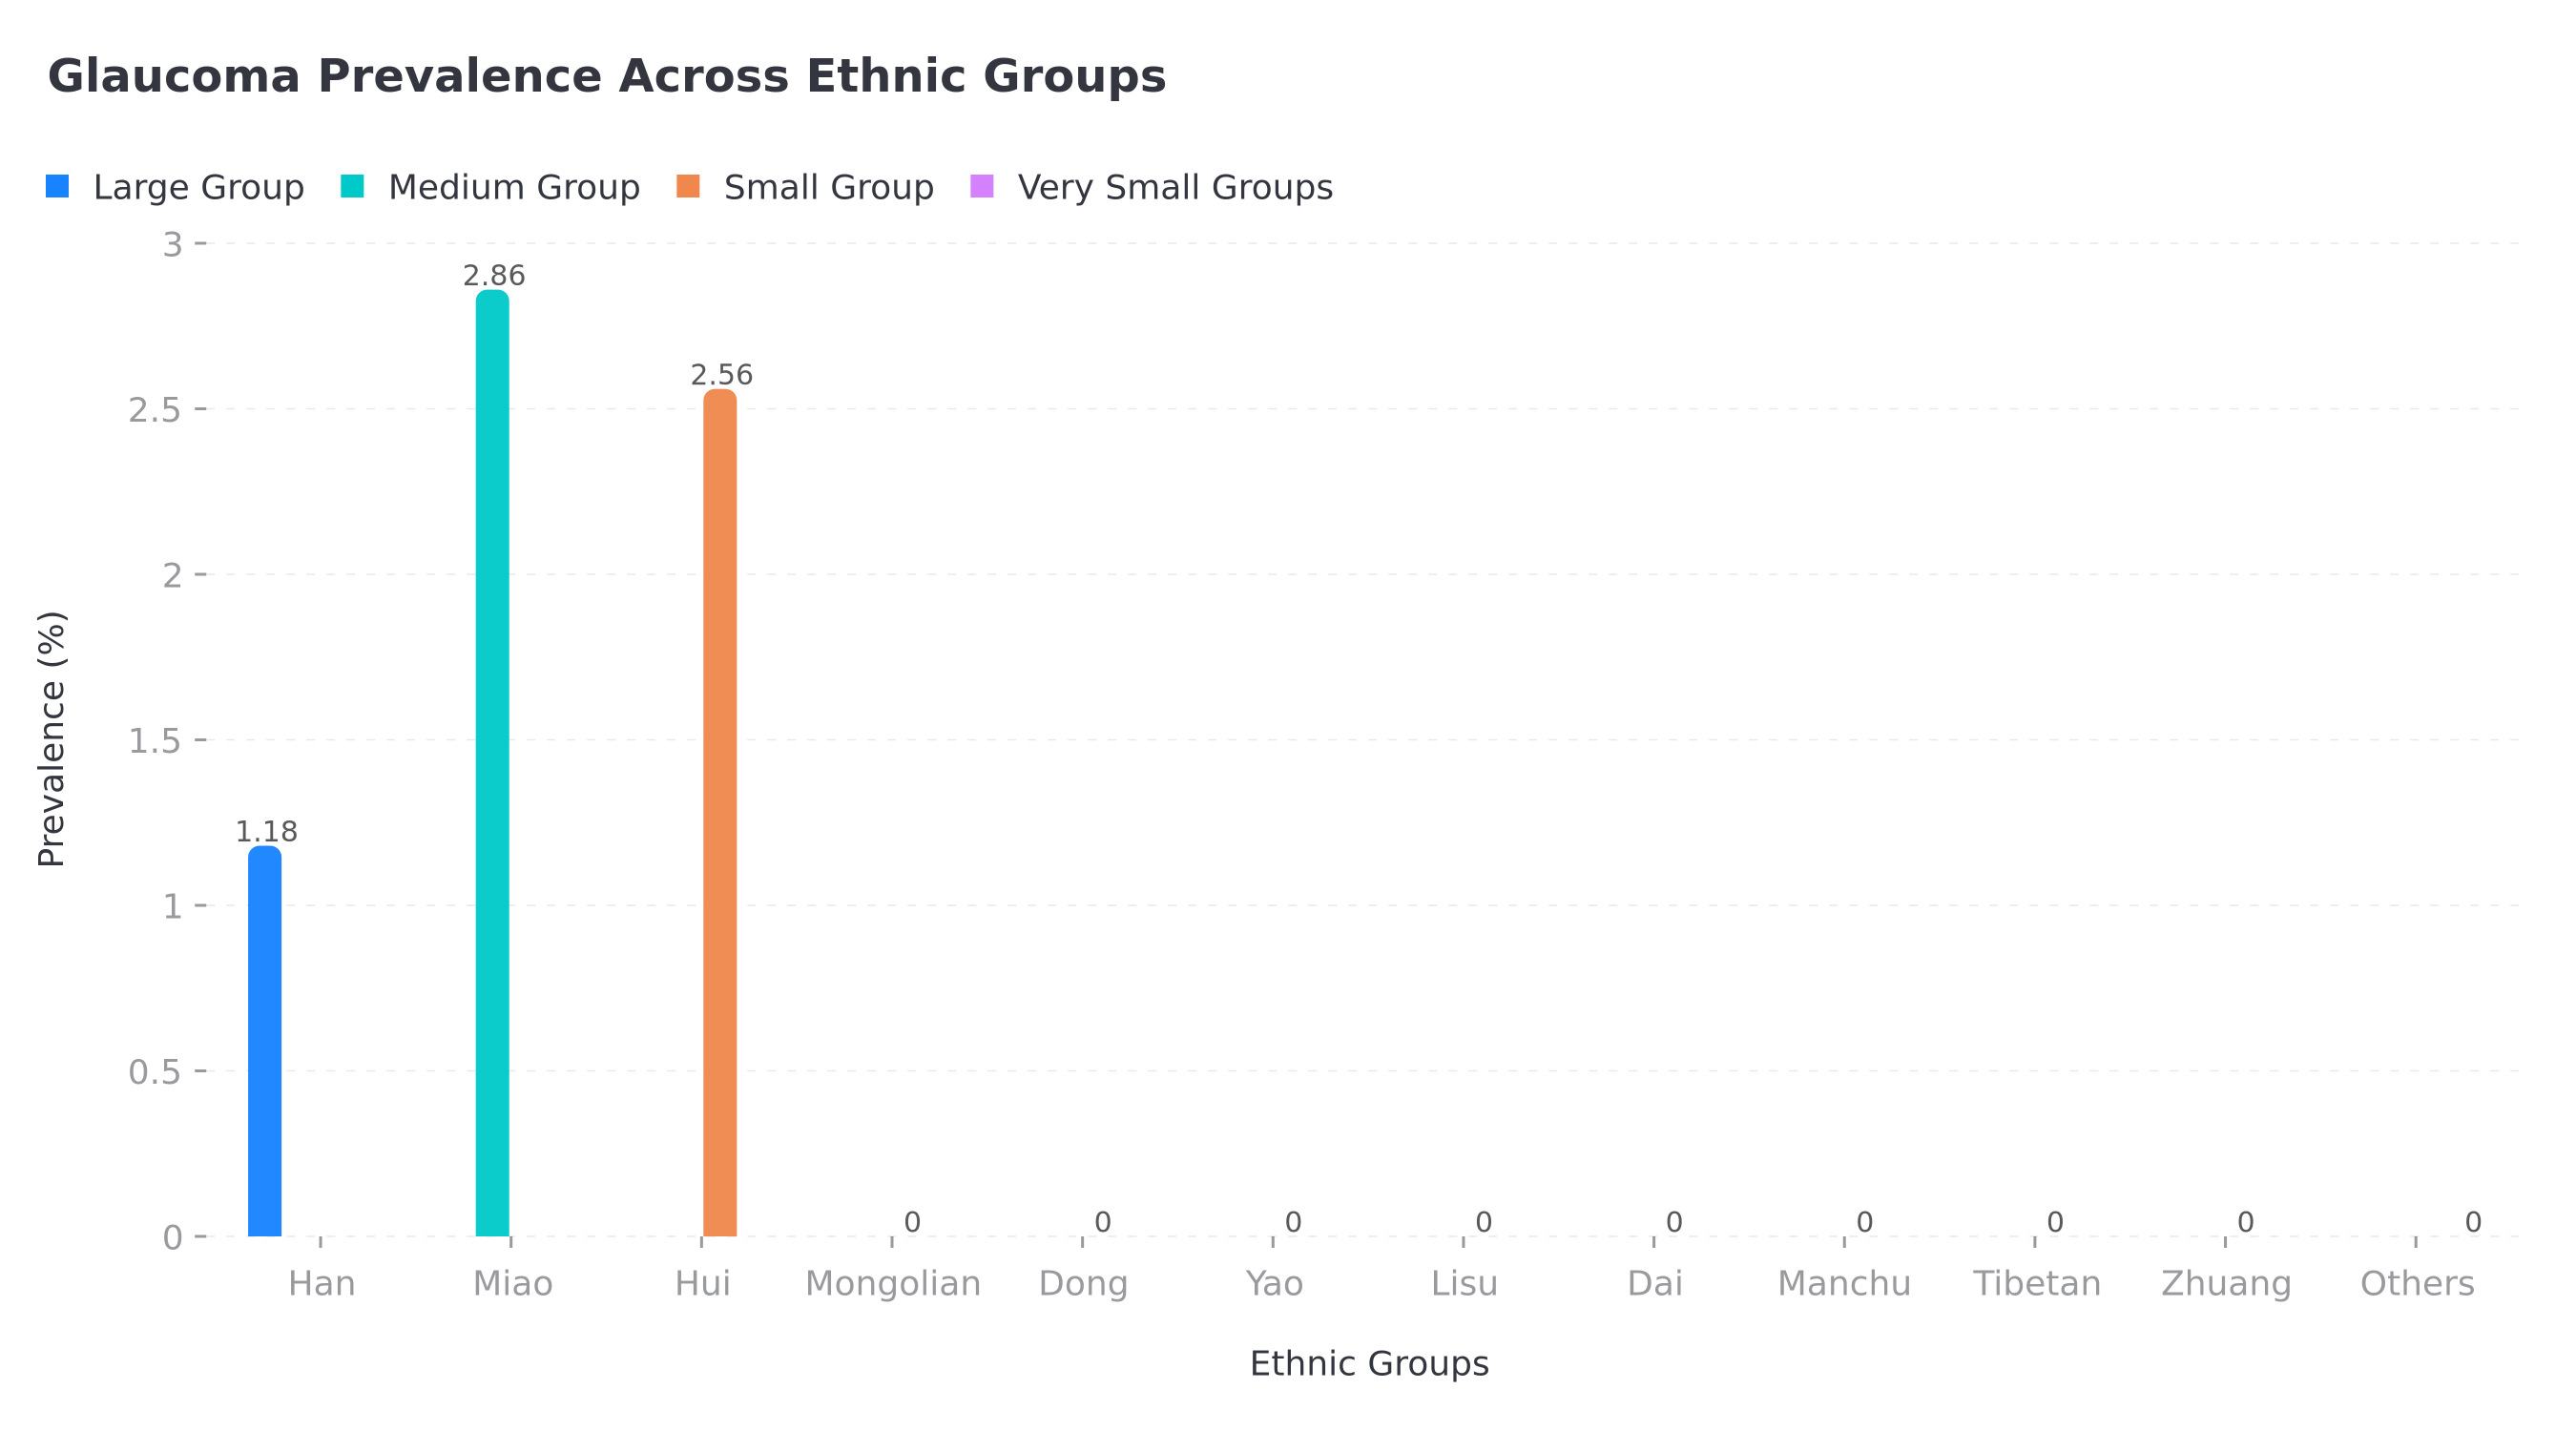
\includegraphics[width=1.2\textwidth]{all/interactive_chart_glaucoma.png}

\end{figure}

\subsection{年龄相关性黄斑变性 | Age-related Macular Degeneration}

总体患病率:0.91\% | Overall prevalence: 0.91\%

\textbf{显著发现 | Notable Findings:}
\begin{itemize}
    \item 种族群体11:8.33\%(2/24例)- 比总体人群高9.2倍*
    
    Ethnic Group 11: 8.33\% (2/24 cases) - 9.2x higher than overall population*
    
    \item 种族群体3:2.56\%(95\% CI: 0.45\%-13.18\%)- 比总体人群高2.8倍
    
    Ethnic Group 3: 2.56\% (95\% CI: 0.45\%-13.18\%) - 2.8x higher than overall population
    
    \item 种族群体8:2.13\%(95\% CI: 0.73\%-6.07\%)- 比总体人群高2.3倍
    
    Ethnic Group 8: 2.13\% (95\% CI: 0.73\%-6.07\%) - 2.3x higher than overall population
\end{itemize}

\textit{*由于样本量小需谨慎解释 | *Interpret with caution due to small sample size}

\begin{figure}[H]
\hspace{-2cm}
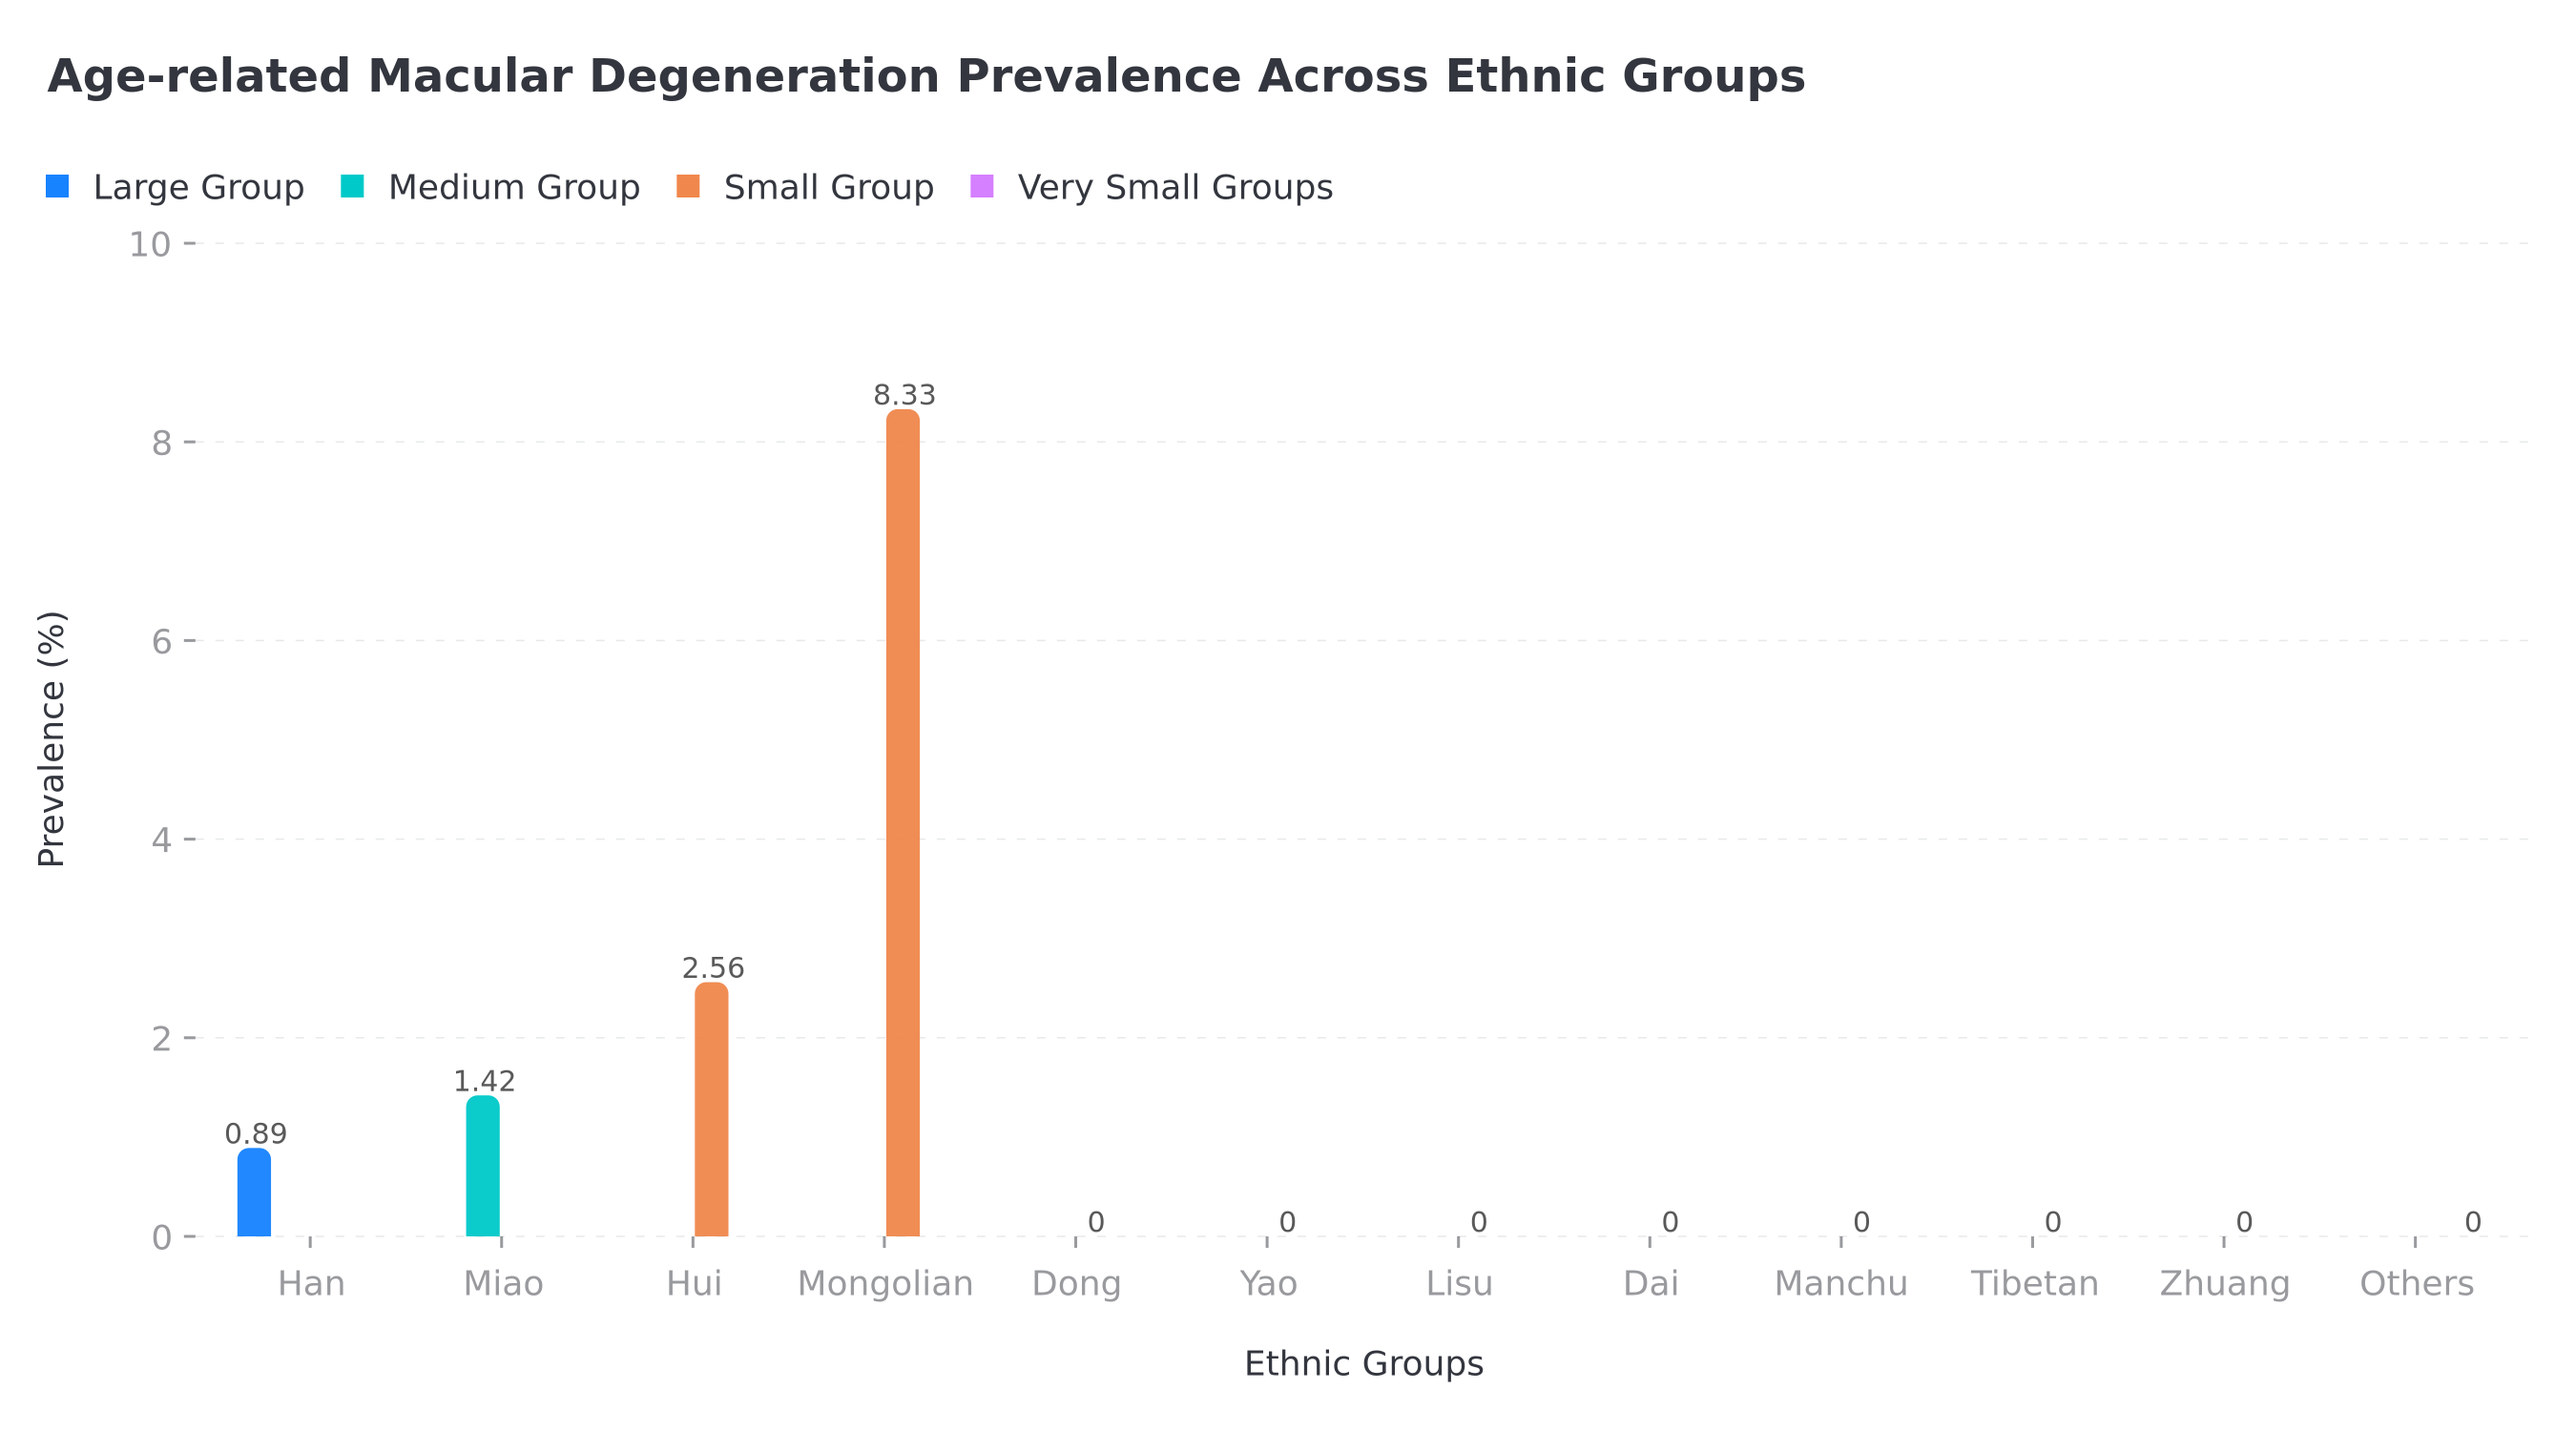
\includegraphics[width=1.2\textwidth]{all/interactive_chart_amd.png}
\end{figure}


\subsection{外周动脉疾病症状 | Peripheral Artery Disease Symptoms}

总体患病率:25.32\% | Overall prevalence: 25.32\%

\textbf{显著发现 | Notable Findings:}
\begin{itemize}
    \item 种族群体19:75.00\%(3/4例)- 比总体人群高3.0倍*
    
    Ethnic Group 19: 75.00\% (3/4 cases) - 3.0x higher than overall population*
    
    \item 种族群体11:33.33\%(8/24例)- 比总体人群高1.3倍*
    
    Ethnic Group 11: 33.33\% (8/24 cases) - 1.3x higher than overall population*
    
    \item 种族群体1:25.51\%(95\% CI: 24.81\%-26.22\%)- 与总体人群相似
    
    Ethnic Group 1: 25.51\% (95\% CI: 24.81\%-26.22\%) - Similar to overall population
    
    \item 种族群体8:7.09\%(95\% CI: 3.84\%-12.73\%)- 比总体人群低0.3倍
    
    Ethnic Group 8: 7.09\% (95\% CI: 3.84\%-12.73\%) - 0.3x lower than overall population
\end{itemize}

\colorbox{yellow}{\parbox{\textwidth}{
\textbf{重要提示 | Important Note:} 这是唯一在多重检验校正后显示统计学显著差异的疾病。

This was the only disease showing statistically significant differences after multiple testing correction.
}}

\begin{figure}[H]
\hspace{-2cm}
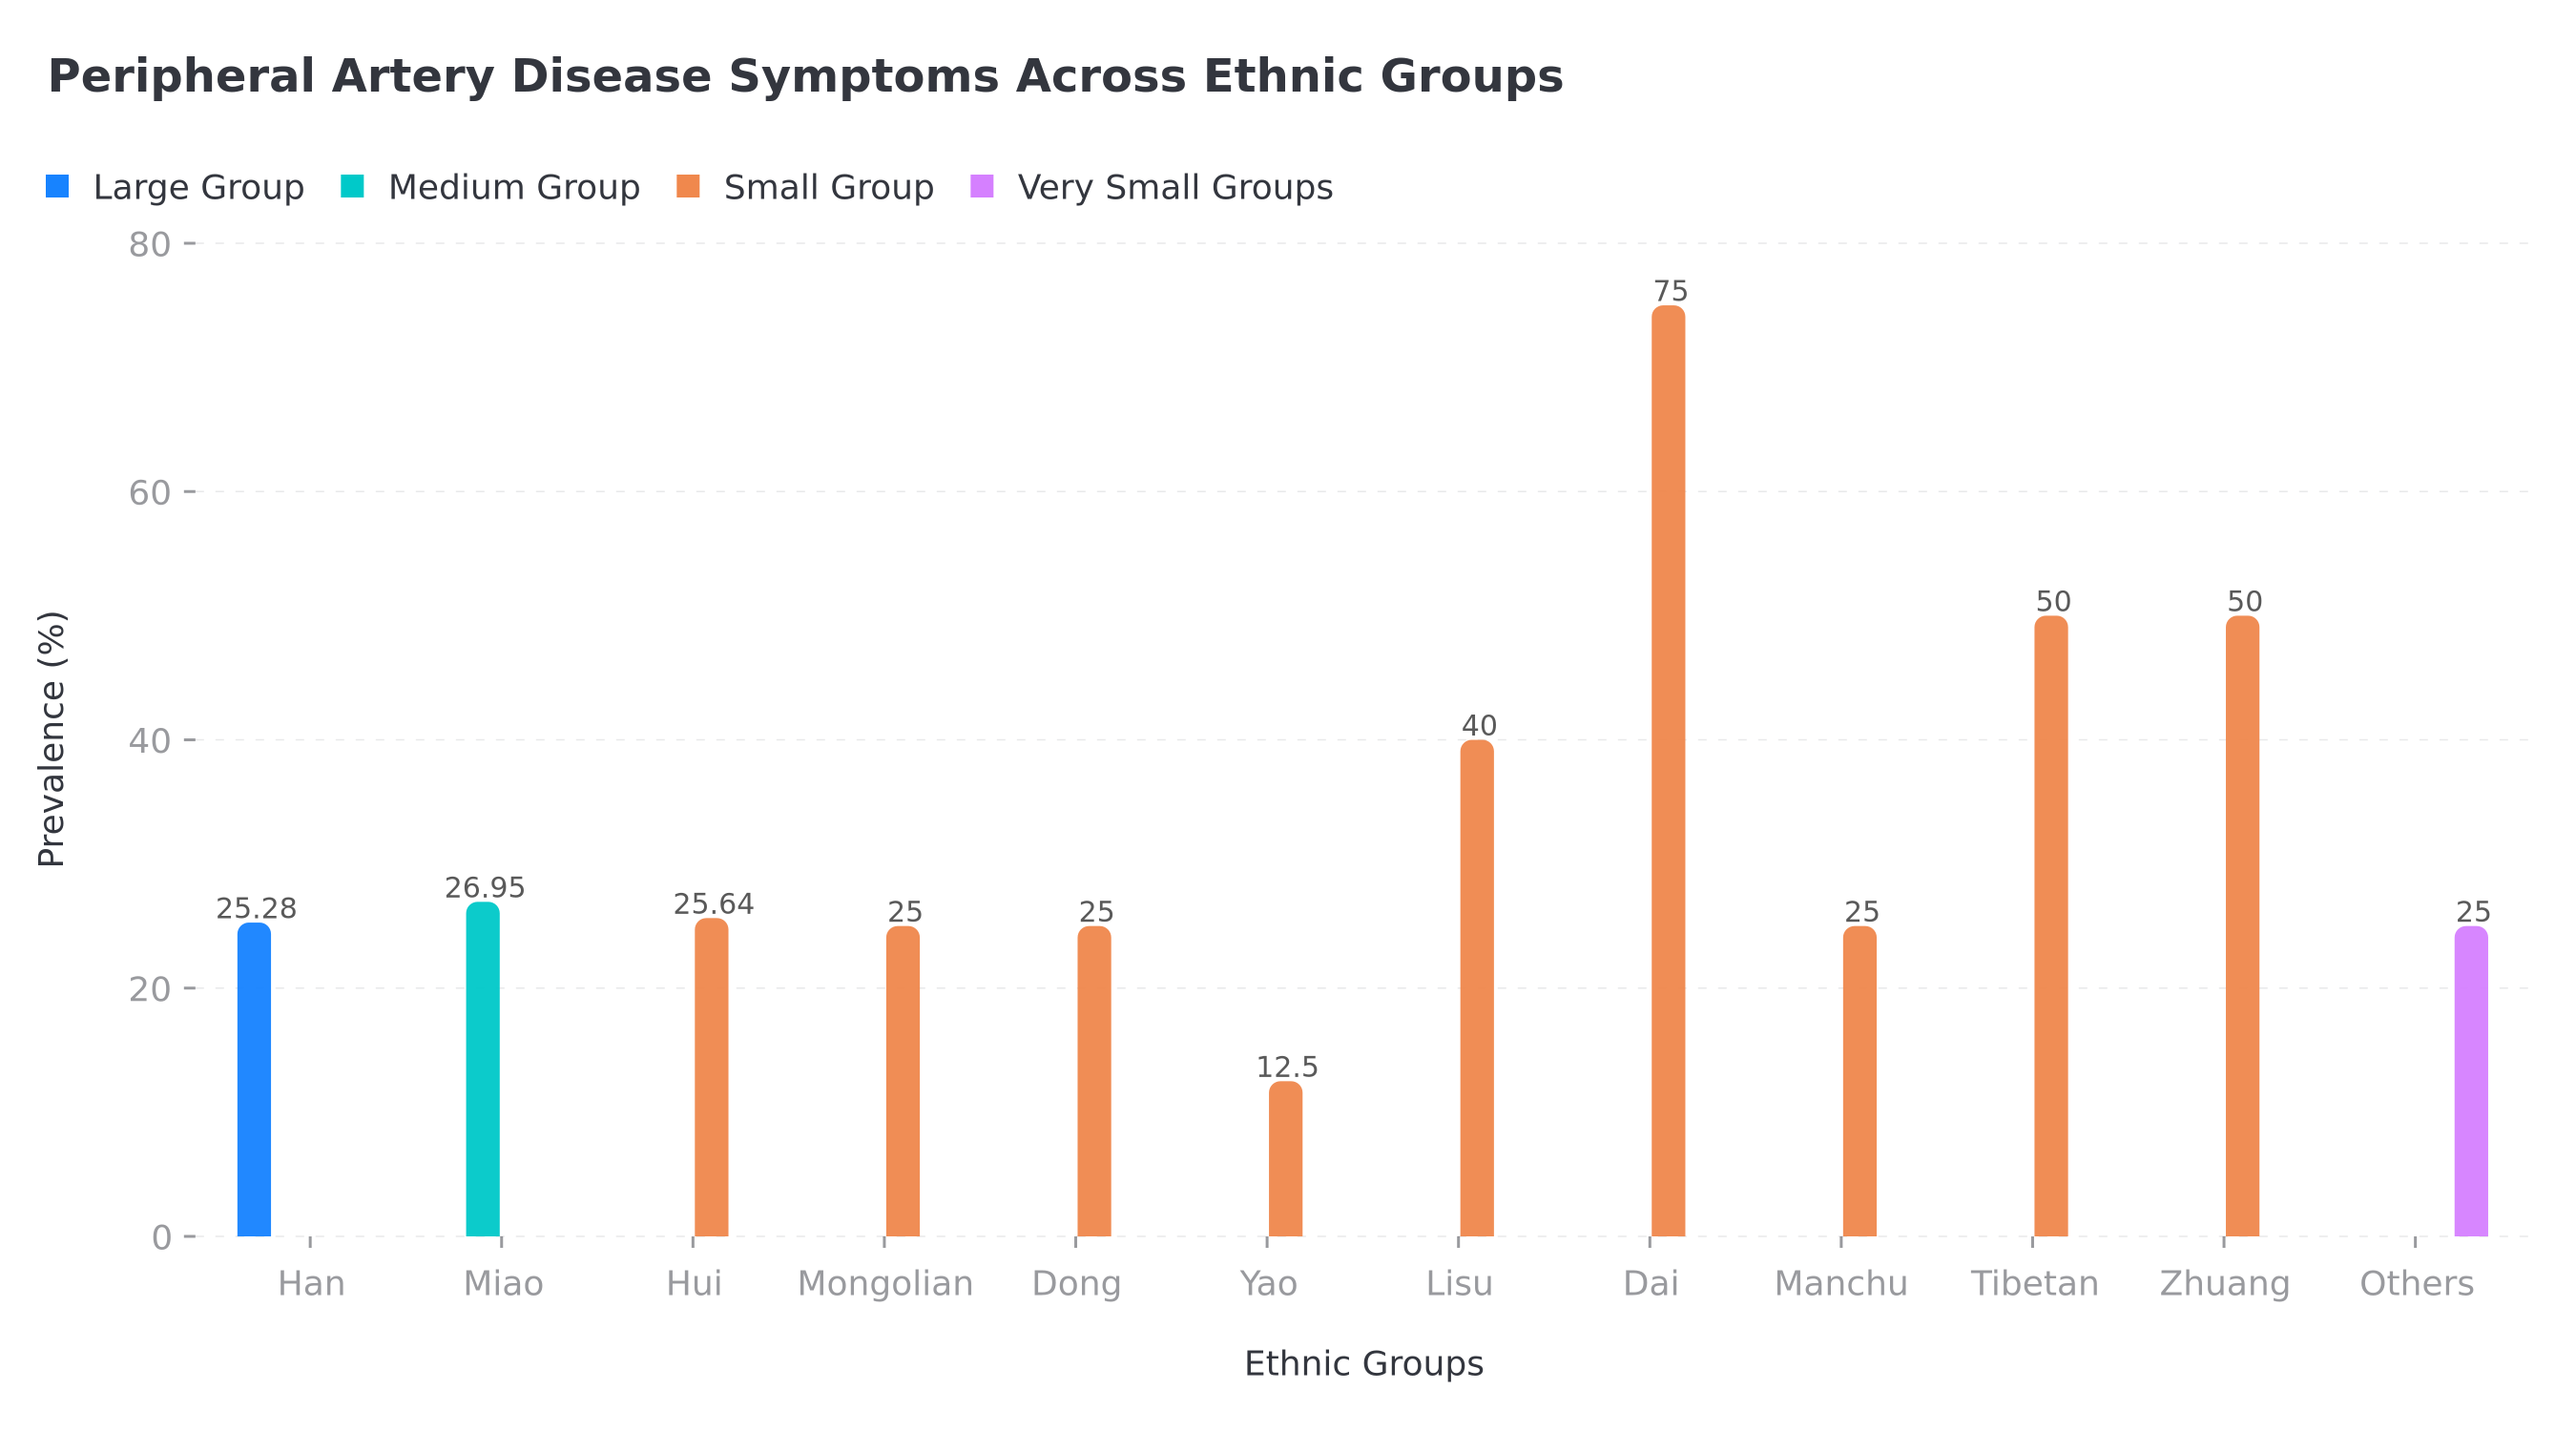
\includegraphics[width=1.2\textwidth]{all/interactive_chart_peripheral_artery_disease.png}
\end{figure}

\section{统计分析 | Statistical Analysis}

\subsection{假设检验 | Hypothesis Testing}

对每种疾病在不同种族群体间进行卡方检验(或小期望计数时使用Fisher精确检验)。

Chi-square tests (or Fisher's exact tests for small expected counts) were performed for each disease across ethnic groups.

\begin{table}[H]
\centering
\caption{原始p值 | Original p-values}
\begin{tabular}{@{}lc@{}}
\toprule
\textbf{疾病 | Disease} & \textbf{p值 | p-value} \\
\midrule
外周动脉疾病症状 | Peripheral Artery Disease Symptoms & 0.00046 \\
缺血性心脏病 | Ischemic Heart Disease & 0.032 \\
糖尿病(临床标准)| Diabetes (Clinical Criteria) & 0.058 \\
早期呼吸道疾病 | Early Life Respiratory Disease & 0.105 \\
年龄相关性黄斑变性 | Age-related Macular Degeneration & 0.187 \\
糖尿病(报告或血液检测)| Diabetes (Reported or Blood Test) & 0.382 \\
白内障 | Cataract & 0.451 \\
青光眼 | Glaucoma & 0.993 \\
\bottomrule
\end{tabular}
\end{table}

\subsection{多重检验校正 | Multiple Testing Correction}

应用Benjamini-Hochberg错误发现率校正:

Benjamini-Hochberg False Discovery Rate correction was applied:

\colorbox{cyan!20}{\parbox{\textwidth}{
\textbf{校正后p值 | Adjusted p-values:} 只有外周动脉疾病症状保持显著性(校正后p = 0.0037)

Only Peripheral Artery Disease Symptoms remained significant (adjusted p = 0.0037)
}}

\section{年龄调整分析 | Age-Adjusted Analysis}

\subsection{标准化患病率比(SPR)| Standardized Prevalence Ratios (SPR)}

年龄调整揭示了重要见解:

Age adjustment revealed important insights:

\begin{table}[H]
\centering
\caption{主要种族群体的标准化患病率比 | Standardized Prevalence Ratios for Major Ethnic Groups}
\begin{tabular}{@{}lccc@{}}
\toprule
\textbf{种族群体 | Ethnic Group} & \textbf{疾病 | Disease} & \textbf{SPR} & \textbf{95\% CI} \\
\midrule
\multirow{3}{*}{群体8 | Group 8 (n=141)} & 外周动脉疾病 | Peripheral Artery Disease & 0.28 & 0.13-0.51 \\
& 青光眼 | Glaucoma & 2.33 & 0.63-5.95 \\
& 年龄相关性黄斑变性 | AMD & 2.39 & 0.49-6.98 \\
\midrule
\multirow{2}{*}{群体3 | Group 3 (n=39)} & 缺血性心脏病 | Ischemic Heart Disease & 2.38 & 0.96-4.90 \\
& 年龄相关性黄斑变性 | AMD & 3.48 & 0.09-19.36 \\
\bottomrule
\end{tabular}
\end{table}

\section{疾病相关性和共病模式 | Disease Correlation and Comorbidity Patterns}

\subsection{疾病相关性 | Disease Correlations}

Pearson相关分析显示疾病间存在适度关联:

Pearson correlation analysis revealed modest associations between diseases:

\textbf{最强相关性 | Strongest Correlations:}
\begin{itemize}
    \item 糖尿病(报告)↔ 糖尿病(临床):r = 0.294
    
    Diabetes (Reported) ↔ Diabetes (Clinical): r = 0.294
    
    \item 白内障 ↔ 缺血性心脏病:r = 0.094
    
    Cataract ↔ Ischemic Heart Disease: r = 0.094
    
    \item 白内障 ↔ 青光眼:r = 0.087
    
    Cataract ↔ Glaucoma: r = 0.087
    
    \item 白内障 ↔ 糖尿病(临床):r = 0.079
    
    Cataract ↔ Diabetes (Clinical): r = 0.079
\end{itemize}

% \subsection{共病负担 | Comorbidity Burden}

% 多种疾病共存分析:

% Analysis of multiple disease occurrence:

% \begin{table}[H]
% \centering
% \caption{主要种族群体的共病分布 | Comorbidity Distribution in Major Ethnic Groups}
% \resizebox{\textwidth}{!}{
% \begin{tabular}{@{}lcccc@{}}
% \toprule
% \textbf{疾病数量 | Number of Diseases} & \multicolumn{2}{c}{\textbf{种族群体1 | Ethnic Group 1 (n=14,992)}} & \multicolumn{2}{c}{\textbf{种族群体8 | Ethnic Group 8 (n=141)}} \\
% \cmidrule(lr){2-3} \cmidrule(lr){4-5}
% & \textbf{人数 | Count} & \textbf{百分比 | \%} & \textbf{人数 | Count} & \textbf{百分比 | \%} \\
% \midrule
% 无疾病 | No diseases & 8,255 & 55.06 & 89 & 63.12 \\
% 1种疾病 | 1 disease & 4,836 & 32.26 & 38 & 26.95 \\
% 2种疾病 | 2 diseases & 1,441 & 9.61 & 12 & 8.51 \\
% 3种以上疾病 | 3+ diseases & 460 & 3.06 & 2 & 1.42 \\
% \bottomrule
% \end{tabular}
% }
% \end{table}

\section{主成分分析 | Principal Component Analysis}

对具有足够样本量的种族群体疾病模式进行PCA分析显示:

PCA of disease patterns across ethnic groups with adequate sample sizes revealed:

\begin{itemize}
    \item \textbf{PC1(72.01\%方差)}:主要由糖尿病患病率驱动,与呼吸道疾病呈负相关
    
    \textbf{PC1 (72.01\% variance):} Primarily driven by diabetes prevalence and inversely by respiratory disease
    
    \item \textbf{PC2(27.99\%方差)}:主要由外周动脉疾病症状驱动
    
    \textbf{PC2 (27.99\% variance):} Primarily driven by peripheral artery disease symptoms
\end{itemize}

这表明不同种族群体间存在两种主要的疾病聚集模式。

This suggests two major patterns of disease clustering across ethnic groups.

\section{临床意义和建议 | Clinical Implications and Recommendations}

\subsection{针对性筛查的高优先级群体 | High-Priority Groups for Targeted Screening}

基于升高的标准化患病率比:

Based on elevated standardized prevalence ratios:

\begin{table}[H]
\centering
\caption{高风险群体筛查建议 | Screening Recommendations for High-Risk Groups}
\begin{tabular}{@{}p{4cm}p{6cm}p{4cm}@{}}
\toprule
\textbf{种族群体 | Ethnic Group} & \textbf{建议筛查疾病 | Recommended Screening} & \textbf{备注 | Notes} \\
\midrule
种族群体8 | Ethnic Group 8 & 青光眼、年龄相关性黄斑变性 | Glaucoma, Age-related Macular Degeneration & 考虑遗传或环境因素 | Consider genetic/environmental factors \\
\midrule
种族群体3 | Ethnic Group 3 & 缺血性心脏病、年龄相关性黄斑变性 | Ischemic Heart Disease, AMD & 需要进一步调查 | Warrants further investigation \\
\bottomrule
\end{tabular}
\end{table}

\subsection{研究局限性 | Study Limitations}

\begin{enumerate}
    \item \textbf{样本量不平衡 | Sample Size Imbalance}:98.42\%的参与者属于种族群体1,严重限制了少数群体比较的统计效力
    
    98.42\% of participants belong to Ethnic Group 1, severely limiting statistical power for minority group comparisons
    
    \item \textbf{小样本量 | Small Sample Sizes}:15个种族群体中有12个n < 30,使可靠的统计推断具有挑战性
    
    12 of 15 ethnic groups have n < 30, making reliable statistical inference challenging
    
    \item \textbf{多重比较 | Multiple Comparisons}:尽管进行了校正,大量检验增加了虚假发现的风险
    
    Despite correction, the large number of tests increases the risk of spurious findings
    
    \item \textbf{缺失数据 | Missing Data}:原始样本中约38.8\%缺少种族群体数据
    
    Approximately 38.8\% of original sample had missing ethnic group data
\end{enumerate}

\subsection{未来研究建议 | Recommendations for Future Research}

\begin{enumerate}
    \item \textbf{过度抽样 | Oversampling}:未来研究应对少数种族群体进行过度抽样以获得足够的统计效力
    
    Future studies should oversample minority ethnic groups to achieve adequate statistical power
    
    \item \textbf{遗传学研究 | Genetic Studies}:调查可能解释特定种族群体疾病风险升高的遗传标记
    
    Investigate genetic markers that may explain elevated disease risk in specific ethnic groups
    
    \item \textbf{环境因素 | Environmental Factors}:检查可能导致种族差异的社会经济、饮食和生活方式因素
    
    Examine socioeconomic, dietary, and lifestyle factors that may contribute to ethnic disparities
    
    \item \textbf{纵向设计 | Longitudinal Design}:实施前瞻性队列研究以建立时间关系
    
    Implement prospective cohort studies to establish temporal relationships
    
    \item \textbf{验证研究 | Validation Studies}:在种族群体代表性更好的独立队列中重复发现
    
    Replicate findings in independent cohorts with better ethnic group representation
\end{enumerate}

\section{结论 | Conclusions}

这项综合分析揭示了不同种族群体间疾病患病率的显著差异,尽管解释受到严重样本量不平衡的限制。外周动脉疾病症状显示了种族差异的最有力证据,种族群体1显示较高患病率,而种族群体8在年龄调整后显示保护效应。

This comprehensive analysis reveals significant variations in disease prevalence across ethnic groups, though interpretation is limited by severe sample size imbalances. Peripheral Artery Disease Symptoms showed the most robust evidence of ethnic variation, with Ethnic Group 1 showing higher prevalence and Ethnic Group 8 showing protective effects after age adjustment.

虽然几个少数种族群体在各种疾病中显示出显著升高的患病率,但这些发现需要在更大、更平衡的队列中进行验证。识别出的高风险群体,特别是种族群体8和3,需要有针对性的公共卫生干预和对潜在机制的进一步调查。

While several minority ethnic groups showed dramatically elevated prevalence for various conditions, these findings require validation in larger, more balanced cohorts. The identification of high-risk groups, particularly Ethnic Groups 8 and 3, warrants targeted public health interventions and further investigation into underlying mechanisms.

研究人群中种族群体1的强势主导地位突出了更具包容性的研究设计的关键需求,以充分代表种族多样性,从而有效解决健康差异问题。

The strong predominance of Ethnic Group 1 in the study population highlights the critical need for more inclusive research designs that adequately represent ethnic diversity to address health disparities effectively.

\vspace{1cm}


\begin{appendix}
\section{附录 | Appendix}

\begin{figure}[H]
+\hspace{-2cm}
+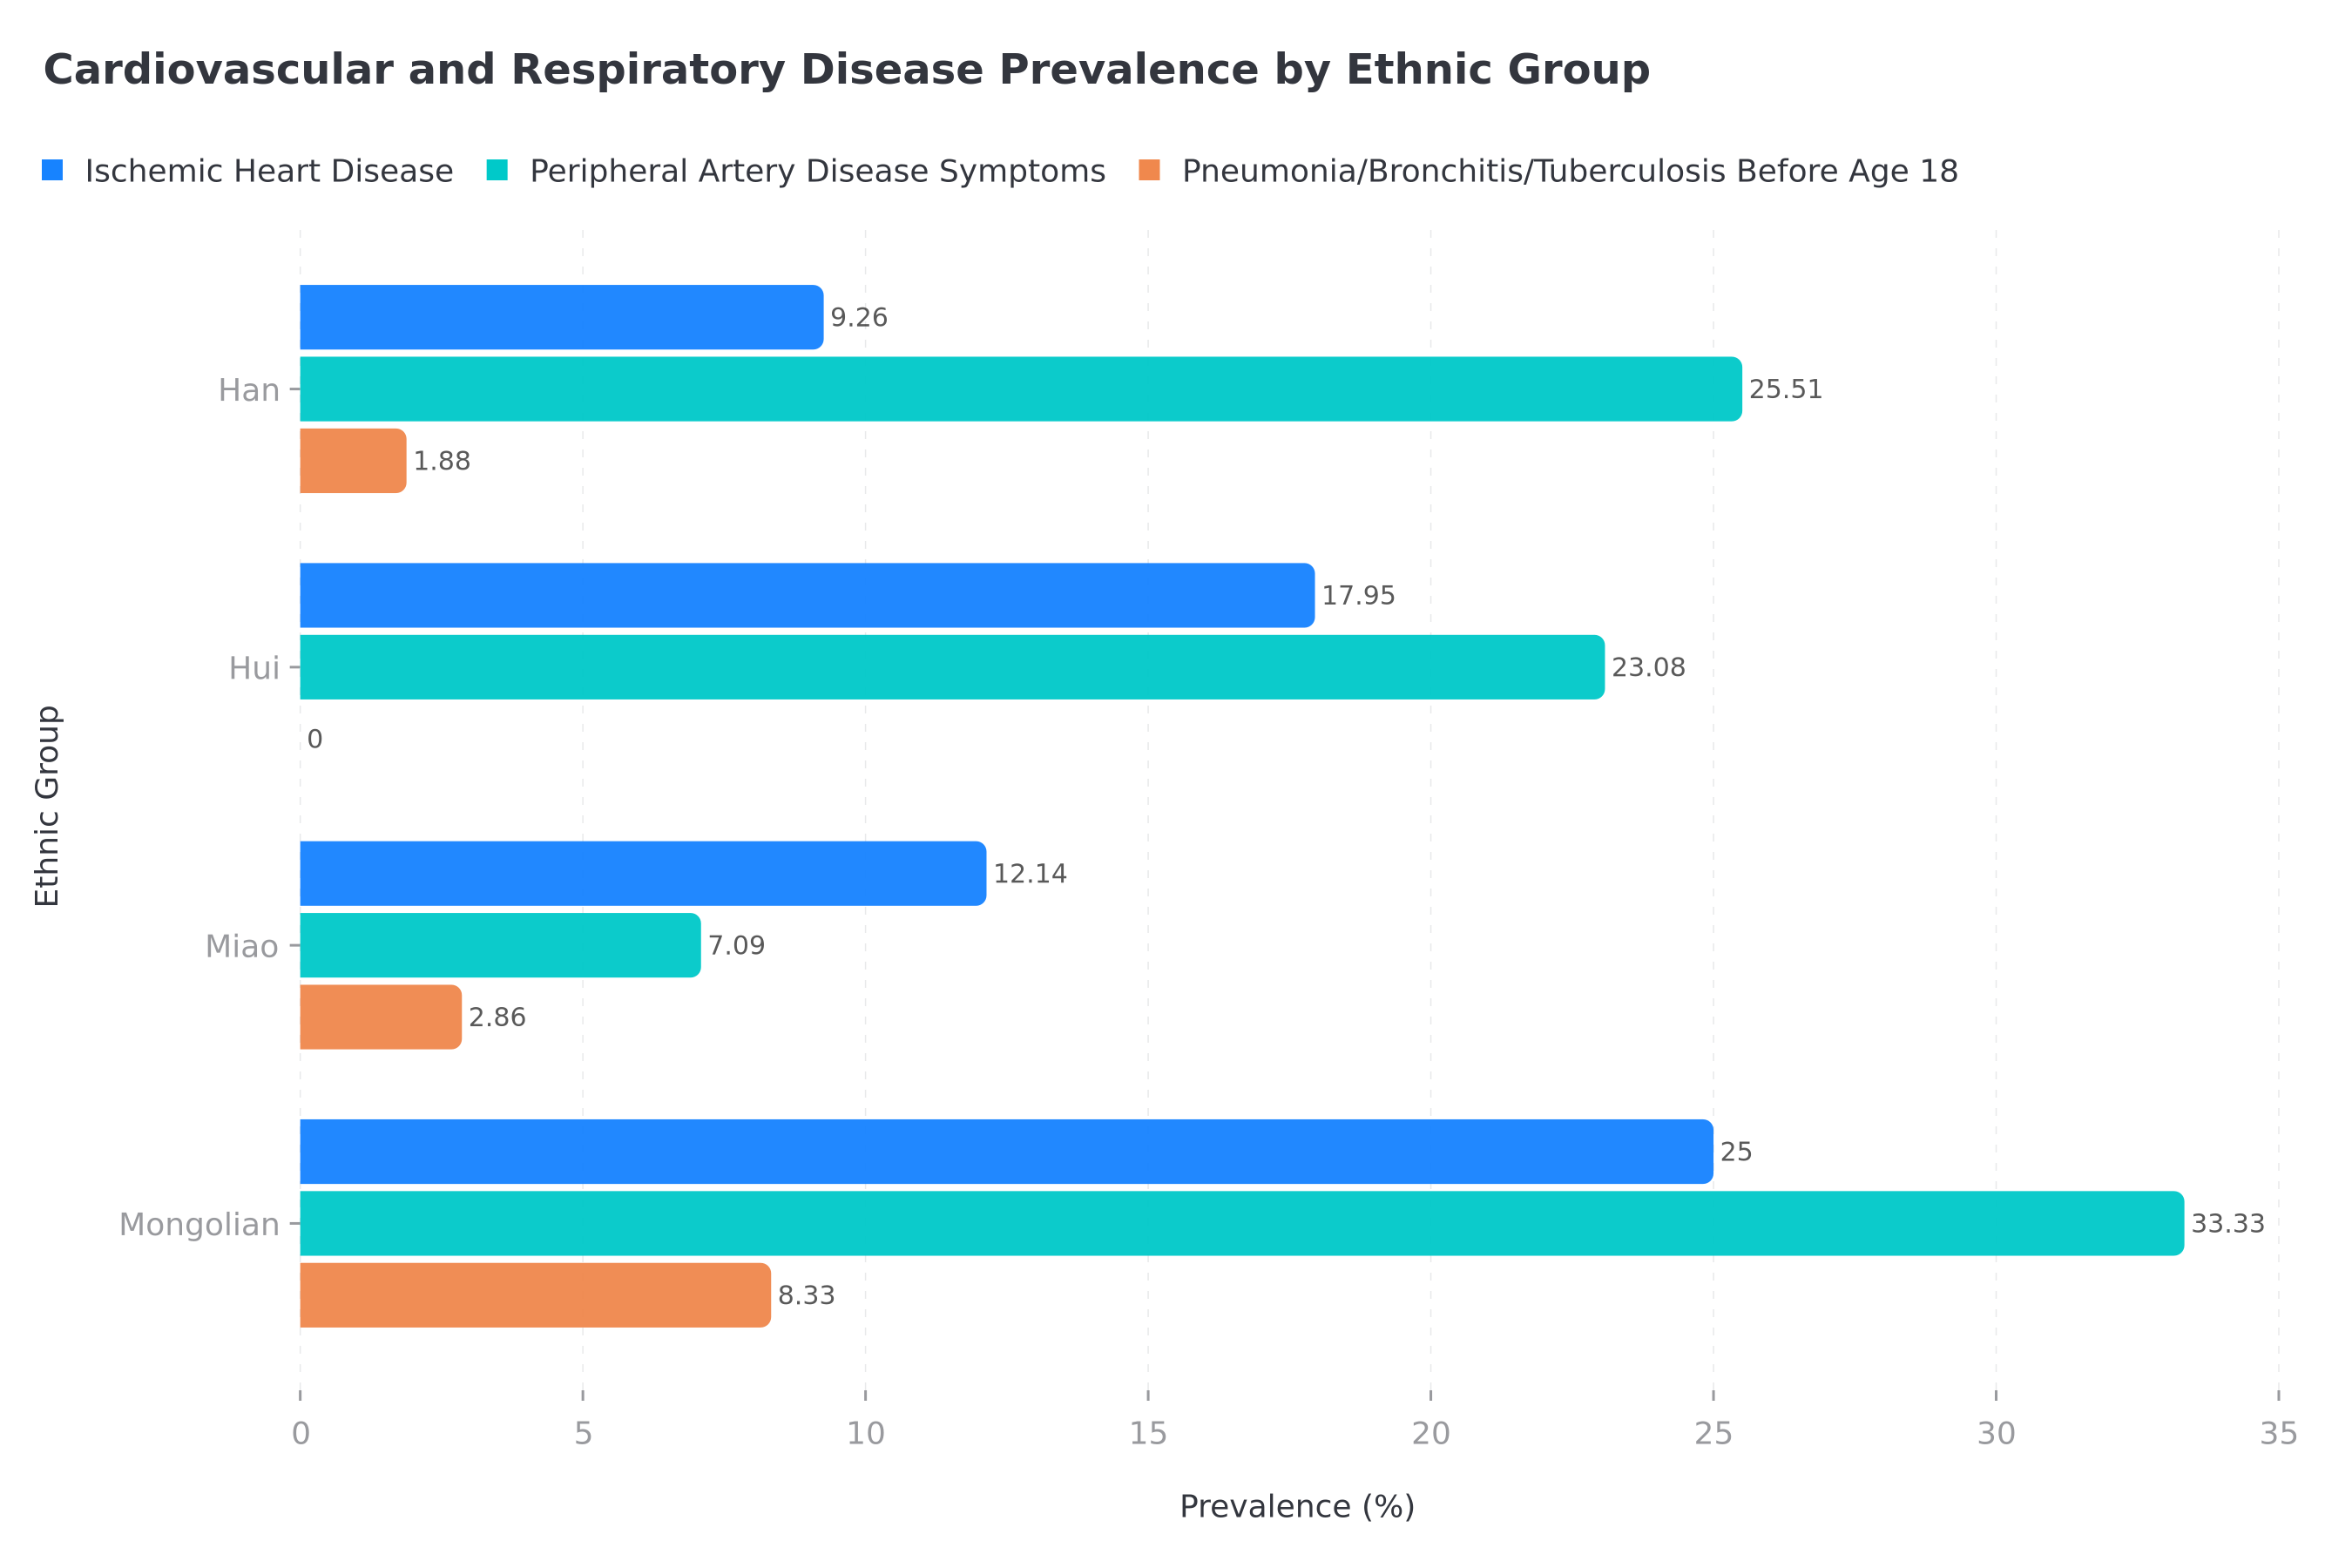
\includegraphics[width=1.2\textwidth]{only_big/cardiovascular_disease_bar_chart.png}
\end{figure}

\begin{figure}[H]
+\hspace{-2cm}
+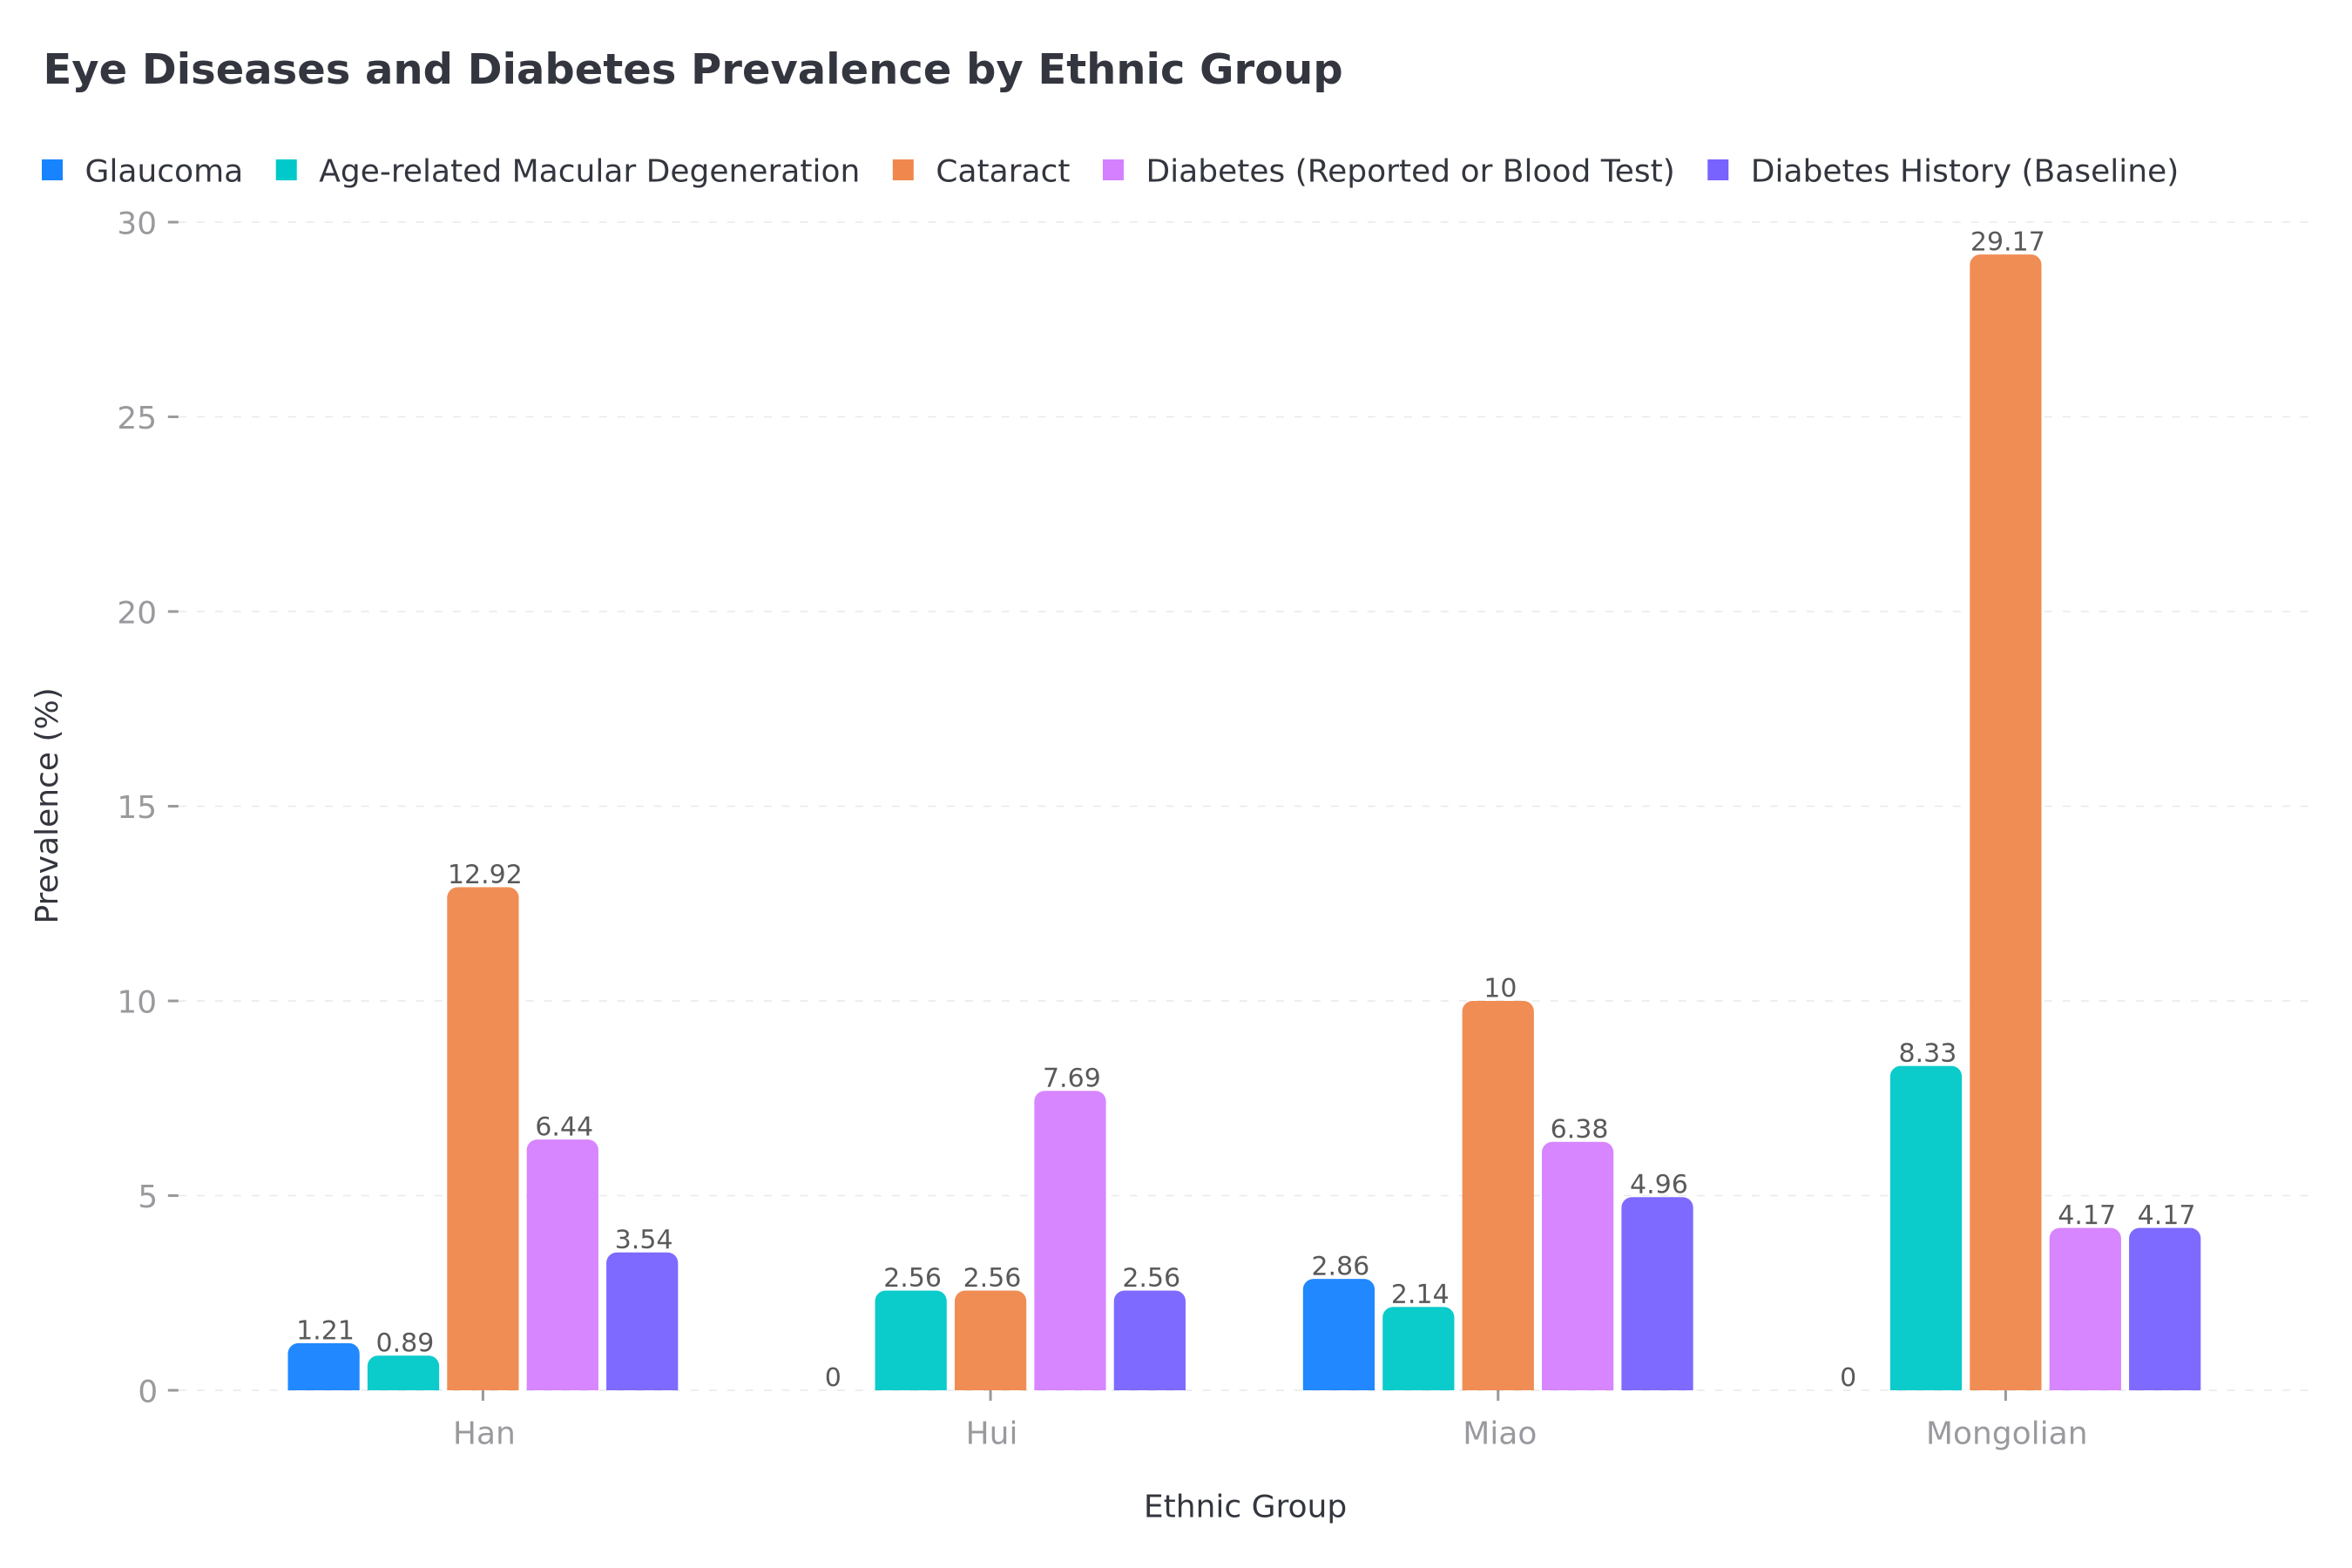
\includegraphics[width=1.2\textwidth]{only_big/eye_disease_column_chart.png}
\end{figure}



\end{appendix}


\begin{center}
\fbox{\begin{minipage}{0.8\textwidth}
\centering
\textbf{报告编制信息 | Report Information}

\vspace{0.5cm}

\begin{tabular}{ll}
\textbf{报告编制日期 | Report Date:} & \today \\
\textbf{分析参与者总数 | Total Participants:} & 15,233 \\
\textbf{有效种族群体 | Valid Ethnic Groups:} & 15 \\
\textbf{分析疾病数量 | Diseases Analyzed:} & 8 \\
\end{tabular}

\vspace{0.5cm}

\textbf{统计方法 | Statistical Methods:}\\
卡方检验/Fisher精确检验配合Benjamini-Hochberg校正、\\
标准化患病率比、主成分分析\\
Chi-square/Fisher's exact tests with Benjamini-Hochberg correction,\\
Standardized Prevalence Ratios, Principal Component Analysis
\end{minipage}}
\end{center}

\end{document} 